\section{Implementation of NF Chaining in Kernel}
I implemented a prototype of per packet NF chaining mechanism in the kernel space. This includes identification of flow, NF chaining system and implementation of two NFs, DoS attack denial and DNAT. 

\subsection{Environment of Implementation}
For the implementation, VM is used running atop hypervisor. Ubuntu 16.04 LTS (64bit) is used as VM's OS. 

\subsection{Detailed Structure of Table}
As explained in Sec. 4.2.2, identification of flow is done with the help of Filter table. Usually the daemon in the user-space takes the command for iptables and set the specified rule in the kernel space. Instead of this, I made a kernel module that is responsible for inserting rule in the Filter table. 

Table is a contiguous memory region where rules and targets are inserted. Every network namespace (ns) has its own tables. Specifically, struct net that represents ns, has struct netns\_ipv4 member, which contains pointers to each table. All tables (from Filter to NAT table) are the same struct xt\_table. 

Figure \ref{fig: filter_table} describes the Filter table. The xt\_table struct has ipt\_table\_info struct that includes pointers to the top of each hook's rule. For example, hook\_entry[0] in ipt\_table\_info points to the top of rule in LOCAL\_IN hook. And hook\_entry[1] points to the top in LOCAL\_OUT hook. To sum up, the biggest box in the middle row is the part of the Filter table for LOCAL\_IN hook and the below box is another part for LOCAL\_OUT hook and so the rest of part for other hooks continues. The box that starts with ipt\_entry and finishes with ipt\_entry\_target corresponds to a set of rules and target which were depicted by a small single box in Figure 4.2. 

\begin{figure*}
	\centering
	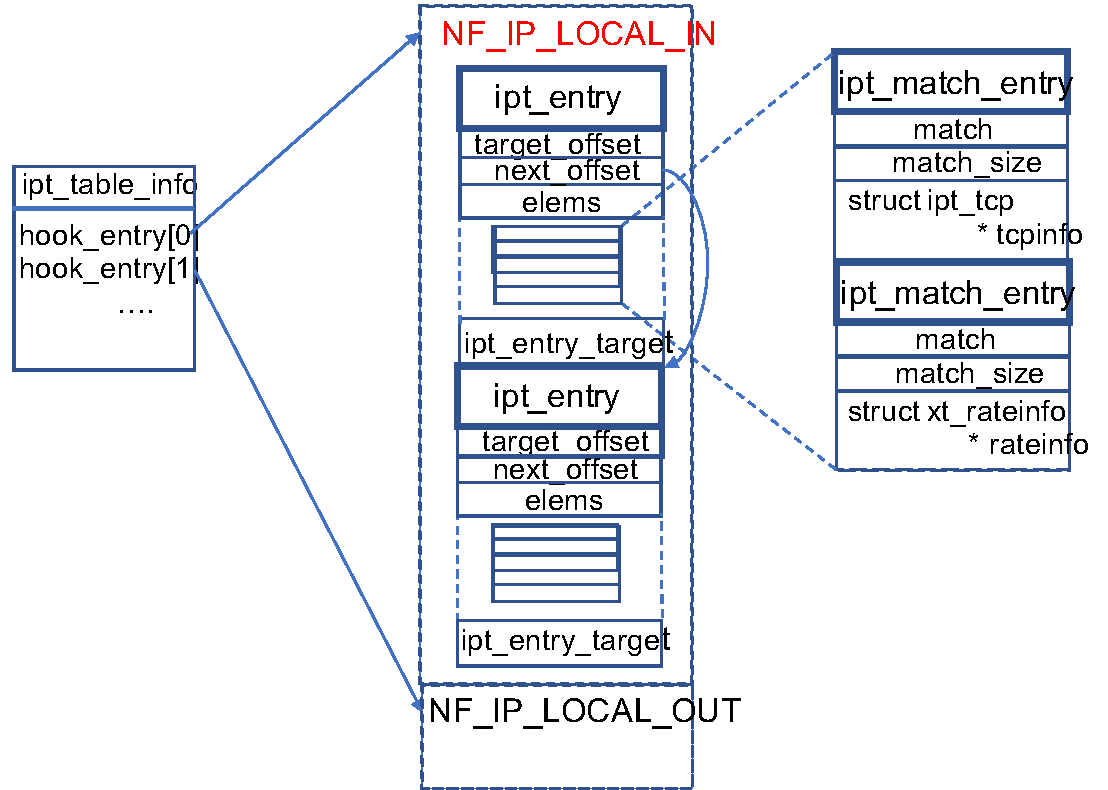
\includegraphics[width=140mm]{pics/filter_table.pdf}
	\caption{Filter Table}
	\label{fig: filter_table}
\end{figure*}

A rule is represented by the following ipt\_entry struct. The ipt\_ip struct member has in\_addr struct to store source and destination IP addresses of the rule. If no rule for IP addresses is specified, they are both initialized to 0.0.0.0. Also a protocol number is set in ipt\_ip struct. target\_offset is the offset to the corresponding target, ipt\_entry\_target struct. And next\_offset is the offset to the next rule, ipt\_entry struct. 

The last member {\tt elems[0]} points to the top of protocol specific rules. A struct ipt\_match\_entry is used to insert specific rules for TCP, UDP, incoming/outgoing devices, etc. Similarly to {\tt ipt\_entry\_target} struct, {\tt ipt\_entry\_match} struct (in Figure \ref{fig: imp4}) has user struct and kernel struct inside a union. {\tt ipt\_match\_entry} struct is organized as following:  In the struct {\tt xt\_match}, a function pointer can be registered to check protocol specific part of the packet. For example, {\tt tcp\_mt} function is registered to check TCP header, such as source / destination port numbers, TCP option and so on. To accommodate various protocol specific rule, {\tt data[0]} is used. For example, TCP specific rules are inserted to {\tt ipt\_tcp} struct and the pointer to this struct is assigned to {\tt data[0]}. Likewise any protocol can be checked. 

Struct {\tt ipt\_entry\_target} is where the information of action (target) against rule match is inserted. Inside {\tt ipt\_entry\_target}, there is a union containing user struct and kernel struct. The former is used when the target has only verdict and no process to be executed. The latter is used when the target has function to  execute. Specifically, the {\tt xt\_target} struct member contains the pointer to the function. In order to realize NF chaining, head of the chain struct {\tt list\_head} is inserted as the last member. So the first two structs in {\tt ipt\_entry\_target} are ignored and only the last struct {\tt list\_head} member is used in case of NF chaining. 

\subsection{Preparation of NF Chaining} 
There are two kernel modules that are responsible for preparing the NF chaining: The first {\tt create\_nfc} module makes NF chains. The second is responsible for setting up rule in Filter table for a chain. Especially struct {\tt ipt\_entry} (in Fig. \ref{fig: imp2}) and struct {\tt ipt\_entry\_target} (in Fig. \ref{fig: imp3}) are used to set rule. 

Before {\tt create\_nfc} module makes a NF chain, kernel modules that forms each NF should be installed in advance. The following information must be provided from the NF : Pointer to the first function of the NF, its priority value, the name of the NF and identification number o f the desired chain (CI). According to this information {\tt create\_nfc} module first of all makes a struct {\tt nf\_target} as described in Figure \ref{fig: imp1}. The provided function pointer is registered in the second member in struct {\tt nf\_target} and so on. If CI is new, a new NF chain is created. Specifically, a new struct {\tt list\_head} is allocated and the {\tt nf\_target} struct is inserted as next node, forming a DLL. If CI already exist, the NF should be inserted in the appropriate existing chain. The priority value in the chain is examined and the the {\tt nf\_target} struct is inserted before the node that has higher priority value.

This second module does roughly three things. 
\begin{itemize}
	\item Setting Rule for NF chain : A rule is set to specify which kind of flow should pass the corresponding NF chain. For IP related rules struct {\tt ipt\_ip} member is set and for protocol specific rule struct {\tt ipt\_match\_entry} that is pointed by {\tt elems[0]} is set. 
	\item Setting the last rule : If none of the set rule for NF chaining matches, the packet will be discarded. To allow packets that are not intended to be processed by any NF chain to go through this system, the last rule is inserted. This rule matches any flow and the target is set as NF\_ACCEPT verdict. 
	\item Registering head of NF chain : After making DLL which forms a NF chain, the head of this DLL is assigned to {\tt list\_head} member in {\tt ipt\_entry\_target} struct. 
\end{itemize}

\begin{figure}
	\begin{center}
		\begin{screen}
			\begin{verbatim}
struct nf_target {
     struct list_head list;
     unsigned int (*nf_func)(struct sk_buff *skb);
     int priority;
     char name[20];
};
			\end{verbatim}	
		\end{screen}
	\end{center}	
	\caption{Struct nf\_target}
	\label{fig: imp1}
\end{figure}

\begin{figure}
	\begin{center}
		\begin{screen}
			\begin{verbatim}
struct ipt_entry {
     struct ipt_ip ip;          // IP related rule
     unsigned int nfcache;
     __u16 target_offset;       // Offset to the corresponding target struct
     __u16 next_offset;         // Offset to the next ipt_entry struct 
     unsigned int comefrom;
     struct xt_counters couters;
     unsigned char elems[0];    // Pointer to region of the protocol-specific rule 
};	
			\end{verbatim}
		\end{screen}
	\end{center}
	\caption{Struct ipt\_entry}
	\label{fig: imp2}
\end{figure}

\begin{figure}
	\begin{center}
		\begin{screen}
			\begin{verbatim}
struct ipt_entry_target {
     union {
            /* Used for user-space daemon to get info */
            struct {
                 __u16 target_size;            // Size of user struct 
                 char name[XT_EXTENSION_MAXNAMELEN];
                 __u8 revision;
            } user;
            /* Used for target with function */
            struct {
                 __u16 target_size;            // Size of kernel struct 
                 struct xt_target *target;     // Function to be executed 
            } kernel;
            __u16 target_size;                 // Size of ipt_entry_target struct 
     } u;
     unsigned char data[0];
     struct list_head *head;     // Pointer to the head of the corresponding DLL
};
			\end{verbatim}
		\end{screen}
	\end{center}
	\caption{Struct ipt\_entry\_target}
	\label{fig: imp3}
\end{figure}
			
\begin{figure}			
	\begin{center}
		\begin{screen}
			\begin{verbatim}
struct ipt_entry_match {
     union {
            /* Used for user-space daemon to get info */
            struct {
                    __u16 match_size;
                    char name[XT_EXTENSION_MAXNAMELEN];
                    __u8 revision;
            } user;
            struct {
                    __u16 match_size;
                    struct xt_match *match;
            } kernel;
            __u16 match_size;
      } u;
      unsigned char data[0];
};
			\end{verbatim}
		\end{screen}
	\end{center}	
	\caption{Struct ipt\_entry\_match}
	\label{fig: imp4}
\end{figure}

\subsection{Implementation of NF Chaining Mechanism}
The PRE\_ROUTING hook is triggered at the end of {\tt ip\_rcv} function (in net/ipv4/ip
\_input.c) in the network stack. The hook eventually calls {\tt ipt\_do\_table} function passing SKB pointer, pointer to struct {\tt xt\_table} as Filter table as arguments. This {\tt ipt\_do\_table} function is in charge of screening rules in the table and taking action specified by the  target. In addition to performing default target process, I added code to practice NF chaining. 

{\tt ipt\_do\_table} function is organized as follows : In the beginning, the first {\tt ipt\_entry} struct  in the table is taken and put in valuable {\tt e}. The SKB is then checked against IP rules ({\tt e -\verb#># ip}). If the rule does not match, the next {\tt ipt\_entry} struct is taken using offset ({\tt e -\verb#># next\_offset}). When matches, SKB is checked against protocol-specific rules ({\tt e -\verb#># ipelems[0]}). If the SKB also pass this second check, it proceeds to processing of target. At this point, {\tt ipt\_entry\_target} struct is taken using offset ({\tt e-\verb#>#target\_offset}) and put in valuable {\tt t}. Depending on the t valuable, there are three ways of action. 
\begin{itemize}
	\item {\tt t -\verb#># u.kernel.target -\verb#># target} is NULL : It means that function is not registered for this target and only a verdict is set. The verdict is obtained by casting {\tt ipt\_entry\_target} to {\tt xt\_standard\_target} struct. 
	\item {\tt t -\verb#># u.kernel.target -\verb#># target} is not NULL : This function is executed and the verdict is returned after the process.   
	\item {\tt t -\verb#># u.user.name} is equal to NFC : This indicates that not the above default targets but the NF chaining is executed. 
\end{itemize}

The code in Figure \ref{fig: nf_chaining_code} describes the detail of NF chaining. The {\tt ipt\_entry\_target} struct {\tt t} has {\tt list\_head} member head, which is the head of the defined NF chain. {\tt t -\verb#># head}'s next node is inserted in {\tt i}. Inside do-while loop, {\tt i} is casted to {\tt nf\_target} struct to get {\tt nf\_func} member. SKB pointer and another value {\tt state} are passed to {\tt nf\_func} function to execute NF's process. After the process a verdict is returned. If verdict equals NF\_DROP, it breaks from the loop and the chaining terminates. Otherwise the next node is taken and the same process continues. 

\begin{figure}
	\begin{center}
		\begin{screen}
			\begin{verbatim}
struct list_head *i;
int verdict = NF_DROP;

if (strncmp(t->u.user.name, "NFC", 3) == 0) {
     i = t->head->next;
     do {
         verdict = ((struct nf_target *)i)->nf_func(skb, state);
         if (verdict == NF_DROP) {
            break;
         } else {
            i = i->next;
         }
     } while (i != t->head);
}
			\end{verbatim}	
		\end{screen}
	\end{center}
	\caption{The NF chaining mechanism in ipt\_do\_table}
	\label{fig: nf_chaining_code}	
\end{figure}

\subsection{Implementation of Network Functions}
I implemented DoS Attack Denial (DAD) and DNAT to practice on NF chaining mechanism.

\begin{figure}
	\begin{center}
		\begin{screen}
			\begin{verbatim}
unsigned int counter_th[10];
struct timespec start_time[10];
unsigned int next_verdict[10], verdict[10];

unsigned int nf_dad_func (struct sk_buff *skb, const struct nf_hook_state *state) 
{
   struct timespec curr_time;
   getnstimeofday(&curr_time);

   for (i = 0; i < 10; i++) {
      if (packet_match(skb, ip[i], port[i])) {
           counter[i]++;
           diff.tv_sec = curr_time.tv_sec - start_time[i].tv_sec;
           if (diff.tv_sec < 10) {
                if (counter[i] > counter_th[i]) {
                     next_verdict[i] = NF_DROP;
                } else {
                     next_verdict[i] = NF_ACCEPT;
                }
                return verdict[i];
           } else {
                getnstimeofday(&start_time[i]);
                verdict[i] = next_verdict[i];
                counter[i] = 0;
                return vredict[i];
          }
      }
   }
}
			\end{verbatim}	
		\end{screen}
	\end{center}
	\caption{Implementation of nf\_dad\_func function for DoS Attack Detection}
	\label{fig: nf_dad_func}
\end{figure}

DAD's aim is to detect sudden increase of traffic and to block the responsible flow. {\tt nf\_dad} (in Fig. \ref{fig: nf_dad_func}) is the function that is registered in {\tt nf\_target} structure. The main idea is that the packet count of a flow in the previous 10 seconds decides whether the flow is dropped or not. 
Every time this function is called, it first set the current time in {\tt curr\_time} value. {\tt ip[i]} and {\tt port[i]} are used to determine the flow ({\tt i} is integer that range from 0 to 9). The "{\tt i}"th flow has its own {\tt start\_time[i]}, which records the last time the measuring started. {\tt counter[i]} values represents the number of received packets per flow since {\tt start\_time[i]}. And {\tt counter\_th[i]} is the threshold of the "{\tt i}"th flow that the dropping of packet is triggered. Each of {\tt verdict[i]} are initialized to NF\_ACCEPT. At first in the iteration, SKB is checked if it matches the "{\tt i}"th flow by {\tt packet\_match} function. If matches, the counter[i] is increased by one. Then elapsed time since {\tt start\_time[i]} is checked whether it is bigger than 10 seconds or not. If it is smaller, {\tt counter[i]} is compared with {\tt counter\_th[i]} and the former exceeds the latter, {\tt next\_verdict[i]}, which is the verdict of next 10 secondes, is set to NF\_DROP. Otherwise it remains NF\_ACCEPT. In both cases {\tt verdict[i]} is returned. If the elapsed time turned bigger than 10 seconds, the {\tt start\_time[i]} is reset to the current time. And the {\tt verdict[i]} for the next 10 seconds is set to {\tt next\_verdict[i]}. 

I used preexisting Netfilter's implementation of NAT for DNAT. NAT (Network Address Translation) is categorized into SNAT (Source NAT) and DNAT (Destination NAT), and both make use of Connection Tracking (CT) system in Netfilter. 

In CT, each SKB is associated with connection tracking information. The process is as follows: Hash is created out of five tuple of SKB and used to look for existing connection represented by struct {\tt nf\_conn}. Struct {\tt nf\_conn} has two tuples representing the flows in two direction, original and reply. If no connection is found for the regarding SKB, a new one is created and connection state is initialized to IP\_CT\_NEW. These two kinds of information (CT info) are set in the SKB for further processing in NAT or other stateful function. If a connection is found by the hash value, it is updated and set in the SKB as well. 

The DNAT process starts from {\tt nf\_nat\_ipv4\_fn} function. It first extracts CT info from the SKB. If the connection state is IP\_CT\_NEW, it screens through the NAT table if there is any action registered for that flow. If a rule matches, the necessary data for SNAT or DNAT is acquired from the table. The data is IP address or port number to which the SKB't header must be changed. From this data, the flow in two directions in struct {\tt nf\_conn} is modified. For example in the case of DNAT, the destination address/port of flow in the original direction and source address/port of flow in the replay direction (reply flow) are changed according to the data. The tuple of replay flow  must be also changed so that when the packet arrives from the changed destination, it can be recognized as replay. After the connection information is set for NAT as mentioned above, packet's header can be changed without looking up the NAT table. This is because the succeeding packets of the same flow first obtains hash value that is used to get the CT info, and according to the tuple in CT info NAT can change the header. To realize such stateful management, NAT is closely tied with the connection tracking system. 



















